% Hier steht der Rezepttitel
\section{Apple mascarpone}
\begin{figure}[H]
  \centering
  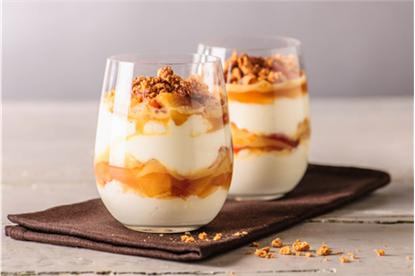
\includegraphics[width=0.45\textwidth]{apfelmasc.jpg}
\end{figure}
% Untertitel
\begin{centering}
% Danach die Zutaten in Tabellenform
% Wie viele werden satt?
\end{centering}
%\textbf{Zutaten:}
\begin{table}[H]
\centering
% eine Tabelle mit insgesamt 4 Spalten, falls mehr Zutaten benoetigt werden
% links: Menge, rechts: Zutat
\begin{tabular*}{1\textwidth}{rlrl}
%& && \\
1.5\,kg & apples & 3\,tbs/1.4 oz & regular sugar \\
2 & cinnamon sticks & 8.8\,oz & mascarpone \\
& cest of one lemon & 5.2\,oz & yogurt \\
6\,tbs & lemon juice & 1.4\,oz & amarettini \\
3\,tbs/1.4 oz & vanilla sugar & & \\
\end{tabular*}
\end{table}
%Zubereitung:

\begin{Notes}

\item Peel apples, cut in quarters, remove the core, and slice into pieces. Combine with cinnamon sticks, lemon cest, 5\,tbs lemon juice, 4\,tbs water, 3\,tbs regular sugar, and 1.5\,tbs vanilla sugar and bring to a boil. Cover and let boil for about 10\,min on medium heat.

\item Put some of the apple pieces aside, purr\'{e}e the rest, add saved pieces back. Let cool.

\item Combine mascarpone, yogurt, 1\,tbs lemon juice, and 1.5\,tbs vanilla sugar and blend well. Crash amarettini and layer with apple purr\'{e}e and cream into glasses.
\end{Notes}
\newpage
% Hier steht der Rezepttitel
\section*{Apfelmascarpone}
\begin{figure}[H]
  \centering
  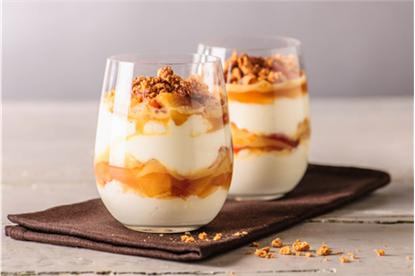
\includegraphics[width=0.45\textwidth]{apfelmasc.jpg}
\end{figure}
% Untertitel
\begin{centering}
% Danach die Zutaten in Tabellenform
% Wie viele werden satt?
\end{centering}
%\textbf{Zutaten:}
\begin{table}[H]
\centering
% eine Tabelle mit insgesamt 4 Spalten, falls mehr Zutaten benoetigt werden
% links: Menge, rechts: Zutat
\begin{tabular*}{1\textwidth}{rlrl}
%& && \\
1,5\,kg & \"{A}pfel & 40\,g & Zucker \\
2 & Zimtstangen & 250\,g & Mascarpone \\
& abgeriebene Schale einer Zitrone & 150\,g & Joghurt \\
6\,EL & Zitronensaft & 40\,g & Amarettini \\
40\,g & Vanillezucker & & \\
\end{tabular*}
\end{table}
%Zubereitung:
\begin{Notes}

\item \"{A}pfel sch\"{a}len, vierteln, entkernen und in St\"{u}cke schneiden. Mit Zimtstangen, Zitronenschale, 5\,EL Zitronensaft, 4\,EL Wasser, 40\,g Zucker und 20\,g Vanillezucker zugedeckt aufkochen und bei mittlerer Hitze ca. 10\,min garen.

\item Einige Apfelst\"{u}cke beiseite stellen, den Rest p\"{u}rieren, die St\"{u}cke wieder untermischen und abk\"{u}hlen lassen.

\item Mascarpone, Joghurt, 1\,EL Zitronensaft und 20\,g Vanillezucker verrühren. Amarettini grob zerstoßen, mit Apfelmus und Creme in Dessertschälchen schichten.

\end{Notes}
\newpage
